\chapter{Part Selection
\index{Chapter!Part Selection}
\index{Part Selection}
\label{Part Selection}}

\begin{figure}[H]
  \centering
  \scalebox{.8}{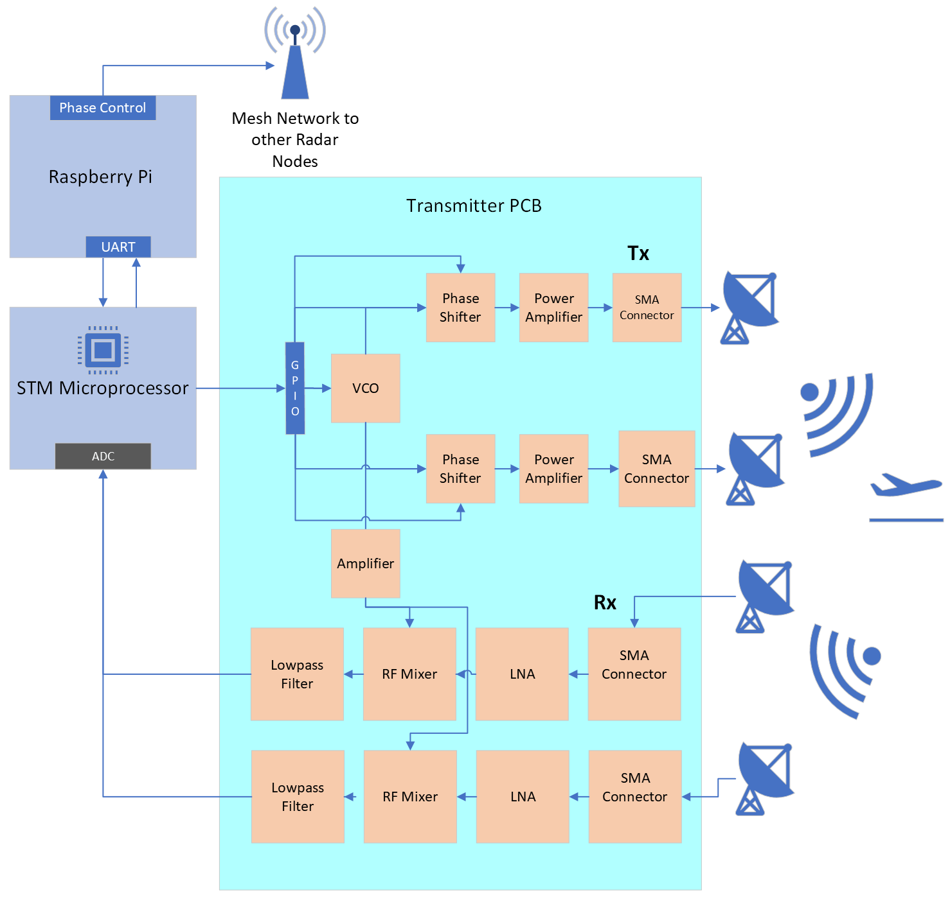
\includegraphics{Diagrams/overview.png}}
\caption{Architecture Overview}
\label{img:projoverview}
\end{figure}

In this chapter, we will go through the architecture of the PCB and show what parts we picked and what purposes they serve.
Figure \ref{img:projoverview} shows the overall architecture of the project.

\section{Voltage Controlled Oscillator (VCO)}
The first step in creating a radar is signal synthesis. You essentially need to create an alternating current signal that can
go through your antenna and radiate out into the air. To reiterate from Chapter \ref{Radar Theory}, higher frequency signals are
important for a better radar resolution, and so it is desired to have a signal that is high in frequency. Naively, at the
beginning of this project we thought we could use a 16 bit DAC to synthesize our signal but after finding out its max clock rate 
was 1 MHz, we realized a DAC was not fit for this. All we needed was something that could create a simple sinusoid at a very
high frequency.

Voltage Controlled Oscillators (VCO) do just this. They take in a "tuning voltage" which corresponds to a certain frequency
of sinusoid which it will output. The circuitry for this is beyond me, but for a good overall guide on VCOs you can check out
DigiKey's article \href{https://www.digikey.com/en/articles/the-basics-of-voltage-controlled-oscillators-vcos}{here}.

Now that we knew how to synthesize our signal, it was important to find a good VCO that had a high output bandwidth. Whatever
bandwidth the VCO has will impact what parts we can get in the other stages of the RF chain since these must be within the VCOs
operating regions. 

\begin{figure}[H]
    \centering
    \scalebox{.7}{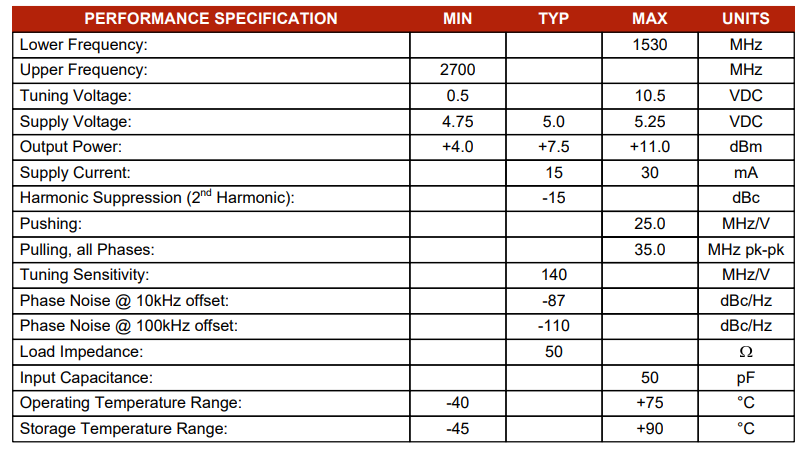
\includegraphics{DatasheetImages/vcotable.png}}
    \caption{VCO Datasheet Table}
    \label{img:vcotable}
\end{figure}
\begin{figure}[H]
    \centering
    \scalebox{.7}{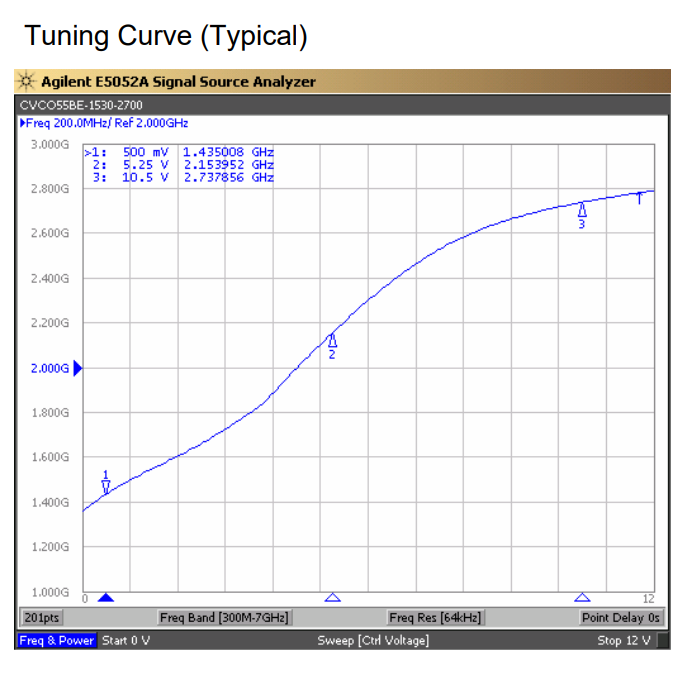
\includegraphics{DatasheetImages/vcotuningtable.png}}
    \caption{Tuning Voltage Graph}
    \label{img:tuninggraph}
\end{figure}

We chose a VCO from Crystek which can be found on Digikey \href{https://www.digikey.com/en/products/detail/crystek-corporation/CVCO55BE-1530-2700/1644030}{here}.
Looking at the specifications table in Figure \ref{img:vcotable}, some good things to look for are first and foremost the frequency
range of the part. It goes from about 1.5-2.7 GHz, which is a pretty wide range and would support a lot of other parts as it also
covers the Wi-Fi band. The second thing to look for is output power. The output power can be a constraint for other parts, since they
might have a absolute limit on their input power, and it is useful to know the output power for finding out how strong your signal will be
once it propogates out of your antenna. Here we can see the output power is around 7.5 dBm, and this will be split four ways. 
Decibels are a logarithmic scale, so we cannot just divide by four but instead use a decibel calculator like \href{https://noisetools.net/decibelcalculator}{this one}.


